%%%%%%%%%%%%%%%%%%%%%%%%%%%%% Preamble %%%%%%%%%%%%%%%%%%%%%%%%%%%%%%%%%%
\begin{center}                                                          %
	\section*{CHAPTER 1}
	\textbf{Name of Chapter 1}                            %
	\setcounter{section}{1}                                             %
	\setcounter{table}{0}                                               %
	\setcounter{figure}{0}                                              %
\end{center}                                                            %
\addcontentsline{toc}{section}{CHAPTER 1 - Name of Chapter 1}           %
\vspace{5mm}                                                            %
%%%%%%%%%%%%%%%%%%%%%%%%%%%%%%%%%%%%%%%%%%%%%%%%%%%%%%%%%%%%%%%%%%%%%%%%%

The Current Setup supports a 5 chapter thesis. To add additional chapters, create a new chapter folder, with a new tex file. Copy and past the preamble above into the new chapters tex file. Update the \\setcounter{number}, to the chapter number. Change both \\section*{} and the \\addcontentsline{toc}{section}{CHANGE} command to the name of the new chapter. Add the chapter in the thesismain.tex file as well.


\cite{IndustEclog}

\subsection{This Is a Chapters Section} %Create Sections within a chapter

%Images can be saved in individual chapter folders and called like this
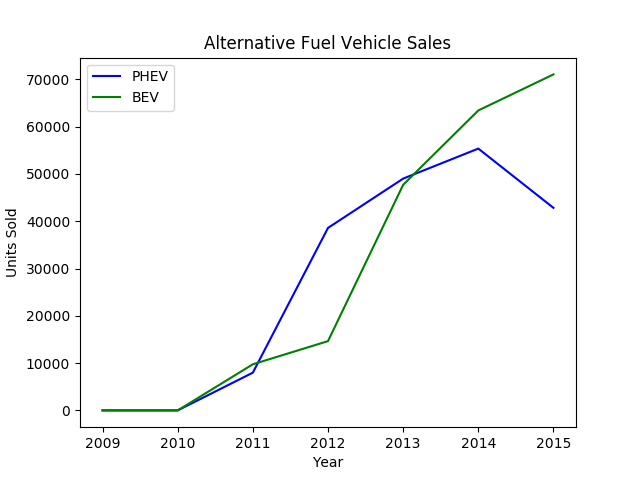
\includegraphics[width=\linewidth]{chapter1/sales}


\subsubsection{This Is a Subsection in a Chapter} %Create a Subsection





  




